\section{Instruction Set}

The processer we made implemented instruction set described in section \ref{sec:instructionset}.
We had the opportunity to expand the instruction set, but we did not see any reason to do so as the limited instruction set made testing easier.

\section{Architecture}

\begin{figure}[ht]
    \centering
    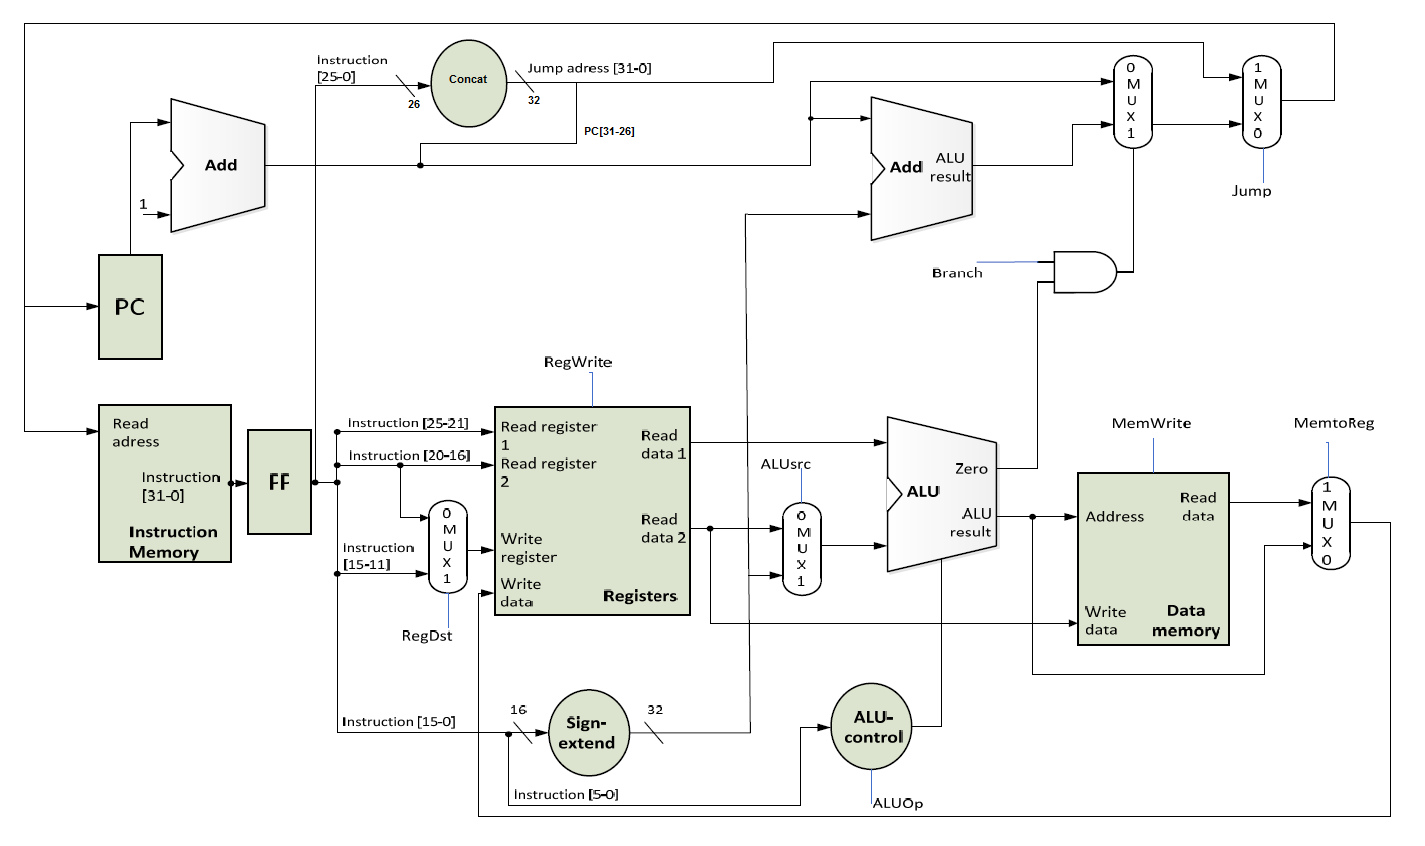
\includegraphics[scale=0.3]{figures/cpu2.png}
    \caption{\label{fig:cpuArchitecture}The implemented CPU architecture.} 
\end{figure}

The CPU architecture closely resembles the suggested one \cite[p.115]{lab-compendium}.
The main difference is that instead of feeding the program counter register into the instruction memory, 
the calculated next program counter is fed into it, and then a flip-flop lets the instruction through at the correct time.

\section{The Control Unit}
\begin{figure}[ht]
    \centering
    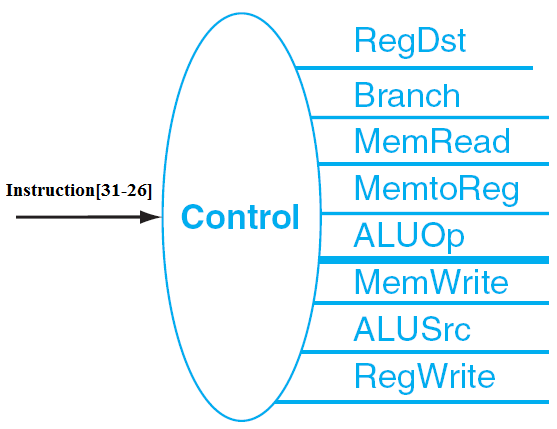
\includegraphics[scale=0.3]{figures/controlunit.png}
    \caption{\label{fig:controlUnit}The control unit.}
\end{figure}

The control unit (CU) was implemented as a state machine, a decoder and a
splitter. On a rising clock edge, it will update the state depending on the
current state. The states, as shown in figure \ref{fig:stateMachine}, are as follow:

\subsection{Fetch}

The instruction is fetched from the instruction memory and the program counter
is updated before the state is set to execute.

\subsection{Execute}

The CU lets the ALU and other logic do its things before setting the state to
that decided by the decoder, which is normally fetch, but stall in case of load
instructions.

\subsection{Stall}

The CU gives the memory an extra cycle to write the data back to the registers,
before setting the state to fetch.

\subsection{Other}

If the CU finds itself in some other state, something weird has gone wrong.
This is only a sanity check, and should never happen.

\begin{figure}[ht] \centering
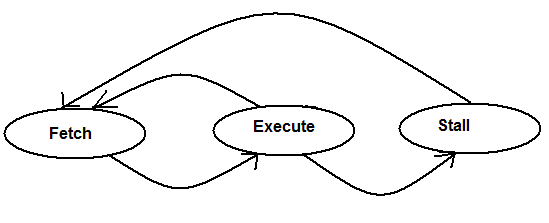
\includegraphics[scale=0.5]{figures/controlunitstatemachine.png}
\caption{\label{fig:stateMachine}The state machine} \end{figure}

\section{Splitter And Decoder}

The splitter simply splits the signal from the instruction memory into its
individual components like opcode, rs, rt, rd and so forth.  The decoder
analyzes the opcode and function signals and enables the correct control signals
and decides the next state.  It is composed of a switch statement with one
condition-block for each opcode.  The R-format has an additional switch
statement to decide the ALU function input.

